% Options for packages loaded elsewhere
\PassOptionsToPackage{unicode}{hyperref}
\PassOptionsToPackage{hyphens}{url}
%
\documentclass[
]{article}
\usepackage{amsmath,amssymb}
\usepackage{lmodern}
\usepackage{iftex}
\ifPDFTeX
  \usepackage[T1]{fontenc}
  \usepackage[utf8]{inputenc}
  \usepackage{textcomp} % provide euro and other symbols
\else % if luatex or xetex
  \usepackage{unicode-math}
  \defaultfontfeatures{Scale=MatchLowercase}
  \defaultfontfeatures[\rmfamily]{Ligatures=TeX,Scale=1}
\fi
% Use upquote if available, for straight quotes in verbatim environments
\IfFileExists{upquote.sty}{\usepackage{upquote}}{}
\IfFileExists{microtype.sty}{% use microtype if available
  \usepackage[]{microtype}
  \UseMicrotypeSet[protrusion]{basicmath} % disable protrusion for tt fonts
}{}
\makeatletter
\@ifundefined{KOMAClassName}{% if non-KOMA class
  \IfFileExists{parskip.sty}{%
    \usepackage{parskip}
  }{% else
    \setlength{\parindent}{0pt}
    \setlength{\parskip}{6pt plus 2pt minus 1pt}}
}{% if KOMA class
  \KOMAoptions{parskip=half}}
\makeatother
\usepackage{xcolor}
\usepackage[margin=1in]{geometry}
\usepackage{color}
\usepackage{fancyvrb}
\newcommand{\VerbBar}{|}
\newcommand{\VERB}{\Verb[commandchars=\\\{\}]}
\DefineVerbatimEnvironment{Highlighting}{Verbatim}{commandchars=\\\{\}}
% Add ',fontsize=\small' for more characters per line
\usepackage{framed}
\definecolor{shadecolor}{RGB}{248,248,248}
\newenvironment{Shaded}{\begin{snugshade}}{\end{snugshade}}
\newcommand{\AlertTok}[1]{\textcolor[rgb]{0.94,0.16,0.16}{#1}}
\newcommand{\AnnotationTok}[1]{\textcolor[rgb]{0.56,0.35,0.01}{\textbf{\textit{#1}}}}
\newcommand{\AttributeTok}[1]{\textcolor[rgb]{0.77,0.63,0.00}{#1}}
\newcommand{\BaseNTok}[1]{\textcolor[rgb]{0.00,0.00,0.81}{#1}}
\newcommand{\BuiltInTok}[1]{#1}
\newcommand{\CharTok}[1]{\textcolor[rgb]{0.31,0.60,0.02}{#1}}
\newcommand{\CommentTok}[1]{\textcolor[rgb]{0.56,0.35,0.01}{\textit{#1}}}
\newcommand{\CommentVarTok}[1]{\textcolor[rgb]{0.56,0.35,0.01}{\textbf{\textit{#1}}}}
\newcommand{\ConstantTok}[1]{\textcolor[rgb]{0.00,0.00,0.00}{#1}}
\newcommand{\ControlFlowTok}[1]{\textcolor[rgb]{0.13,0.29,0.53}{\textbf{#1}}}
\newcommand{\DataTypeTok}[1]{\textcolor[rgb]{0.13,0.29,0.53}{#1}}
\newcommand{\DecValTok}[1]{\textcolor[rgb]{0.00,0.00,0.81}{#1}}
\newcommand{\DocumentationTok}[1]{\textcolor[rgb]{0.56,0.35,0.01}{\textbf{\textit{#1}}}}
\newcommand{\ErrorTok}[1]{\textcolor[rgb]{0.64,0.00,0.00}{\textbf{#1}}}
\newcommand{\ExtensionTok}[1]{#1}
\newcommand{\FloatTok}[1]{\textcolor[rgb]{0.00,0.00,0.81}{#1}}
\newcommand{\FunctionTok}[1]{\textcolor[rgb]{0.00,0.00,0.00}{#1}}
\newcommand{\ImportTok}[1]{#1}
\newcommand{\InformationTok}[1]{\textcolor[rgb]{0.56,0.35,0.01}{\textbf{\textit{#1}}}}
\newcommand{\KeywordTok}[1]{\textcolor[rgb]{0.13,0.29,0.53}{\textbf{#1}}}
\newcommand{\NormalTok}[1]{#1}
\newcommand{\OperatorTok}[1]{\textcolor[rgb]{0.81,0.36,0.00}{\textbf{#1}}}
\newcommand{\OtherTok}[1]{\textcolor[rgb]{0.56,0.35,0.01}{#1}}
\newcommand{\PreprocessorTok}[1]{\textcolor[rgb]{0.56,0.35,0.01}{\textit{#1}}}
\newcommand{\RegionMarkerTok}[1]{#1}
\newcommand{\SpecialCharTok}[1]{\textcolor[rgb]{0.00,0.00,0.00}{#1}}
\newcommand{\SpecialStringTok}[1]{\textcolor[rgb]{0.31,0.60,0.02}{#1}}
\newcommand{\StringTok}[1]{\textcolor[rgb]{0.31,0.60,0.02}{#1}}
\newcommand{\VariableTok}[1]{\textcolor[rgb]{0.00,0.00,0.00}{#1}}
\newcommand{\VerbatimStringTok}[1]{\textcolor[rgb]{0.31,0.60,0.02}{#1}}
\newcommand{\WarningTok}[1]{\textcolor[rgb]{0.56,0.35,0.01}{\textbf{\textit{#1}}}}
\usepackage{graphicx}
\makeatletter
\def\maxwidth{\ifdim\Gin@nat@width>\linewidth\linewidth\else\Gin@nat@width\fi}
\def\maxheight{\ifdim\Gin@nat@height>\textheight\textheight\else\Gin@nat@height\fi}
\makeatother
% Scale images if necessary, so that they will not overflow the page
% margins by default, and it is still possible to overwrite the defaults
% using explicit options in \includegraphics[width, height, ...]{}
\setkeys{Gin}{width=\maxwidth,height=\maxheight,keepaspectratio}
% Set default figure placement to htbp
\makeatletter
\def\fps@figure{htbp}
\makeatother
\setlength{\emergencystretch}{3em} % prevent overfull lines
\providecommand{\tightlist}{%
  \setlength{\itemsep}{0pt}\setlength{\parskip}{0pt}}
\setcounter{secnumdepth}{-\maxdimen} % remove section numbering
\ifLuaTeX
  \usepackage{selnolig}  % disable illegal ligatures
\fi
\IfFileExists{bookmark.sty}{\usepackage{bookmark}}{\usepackage{hyperref}}
\IfFileExists{xurl.sty}{\usepackage{xurl}}{} % add URL line breaks if available
\urlstyle{same} % disable monospaced font for URLs
\hypersetup{
  pdftitle={Modern Applyed Statistics(Chap 11)},
  hidelinks,
  pdfcreator={LaTeX via pandoc}}

\title{Modern Applyed Statistics(Chap 11)}
\author{}
\date{\vspace{-2.5em}}

\begin{document}
\maketitle

\begin{Shaded}
\begin{Highlighting}[]
\FunctionTok{library}\NormalTok{(MASS)}
\end{Highlighting}
\end{Shaded}

\begin{verbatim}
## Warning: 패키지 'MASS'는 R 버전 4.1.3에서 작성되었습니다
\end{verbatim}

\begin{Shaded}
\begin{Highlighting}[]
\FunctionTok{library}\NormalTok{(class)}
\FunctionTok{library}\NormalTok{(fastICA)}
\end{Highlighting}
\end{Shaded}

\begin{verbatim}
## Warning: 패키지 'fastICA'는 R 버전 4.1.3에서 작성되었습니다
\end{verbatim}

\begin{Shaded}
\begin{Highlighting}[]
\FunctionTok{library}\NormalTok{(cluster)}
\FunctionTok{options}\NormalTok{(}\AttributeTok{width=}\DecValTok{65}\NormalTok{, }\AttributeTok{digits=}\DecValTok{5}\NormalTok{)}

\CommentTok{\# install.packages("../package/xgobi\_1.2{-}15.tar.gz", repos = NULL, type = "source")}
\CommentTok{\# install.packages("../package/RGtk2\_2.20.36.tar.gz", repos = NULL, type = "source")}
\CommentTok{\# install.packages("../package/rggobi\_2.1.22.tar.gz", repos = NULL, type = "source")}
\end{Highlighting}
\end{Shaded}

\hypertarget{visualization-methods}{%
\subsection{11.1 Visualization methods}\label{visualization-methods}}

\hypertarget{principal-component-analysis}{%
\subsubsection{1) Principal Component
analysis}\label{principal-component-analysis}}

\begin{Shaded}
\begin{Highlighting}[]
\CommentTok{\# Iris data}
\NormalTok{ir }\OtherTok{\textless{}{-}} \FunctionTok{rbind}\NormalTok{(iris3[,,}\DecValTok{1}\NormalTok{], iris3[,,}\DecValTok{2}\NormalTok{], iris3[,,}\DecValTok{3}\NormalTok{])}
\NormalTok{ir.species }\OtherTok{\textless{}{-}} \FunctionTok{factor}\NormalTok{(}\FunctionTok{c}\NormalTok{(}\FunctionTok{rep}\NormalTok{(}\StringTok{"s"}\NormalTok{, }\DecValTok{50}\NormalTok{), }\FunctionTok{rep}\NormalTok{(}\StringTok{"c"}\NormalTok{, }\DecValTok{50}\NormalTok{), }\FunctionTok{rep}\NormalTok{(}\StringTok{"v"}\NormalTok{, }\DecValTok{50}\NormalTok{)))}

\CommentTok{\# Principal Component for the log{-}transformed iris data.}
\NormalTok{(ir.pca }\OtherTok{\textless{}{-}} \FunctionTok{princomp}\NormalTok{(}\FunctionTok{log}\NormalTok{(ir), }\AttributeTok{cor =} \ConstantTok{TRUE}\NormalTok{))}
\end{Highlighting}
\end{Shaded}

\begin{verbatim}
## Call:
## princomp(x = log(ir), cor = TRUE)
## 
## Standard deviations:
##  Comp.1  Comp.2  Comp.3  Comp.4 
## 1.71246 0.95238 0.36470 0.16568 
## 
##  4  variables and  150 observations.
\end{verbatim}

\begin{Shaded}
\begin{Highlighting}[]
\FunctionTok{summary}\NormalTok{(ir.pca)}
\end{Highlighting}
\end{Shaded}

\begin{verbatim}
## Importance of components:
##                         Comp.1  Comp.2   Comp.3    Comp.4
## Standard deviation     1.71246 0.95238 0.364703 0.1656840
## Proportion of Variance 0.73313 0.22676 0.033252 0.0068628
## Cumulative Proportion  0.73313 0.95989 0.993137 1.0000000
\end{verbatim}

\begin{Shaded}
\begin{Highlighting}[]
\FunctionTok{plot}\NormalTok{(ir.pca)}
\end{Highlighting}
\end{Shaded}

\includegraphics{modern_applied_statistics_CH11_files/figure-latex/unnamed-chunk-2-1.pdf}

\begin{Shaded}
\begin{Highlighting}[]
\CommentTok{\# First two principal components for the log{-}transformed iris data.}
\NormalTok{ir.pc }\OtherTok{\textless{}{-}} \FunctionTok{predict}\NormalTok{(ir.pca)}
\FunctionTok{eqscplot}\NormalTok{(ir.pc[, }\DecValTok{1}\SpecialCharTok{:}\DecValTok{2}\NormalTok{], }\AttributeTok{type =} \StringTok{"n"}\NormalTok{,}
         \AttributeTok{xlab =} \StringTok{"first principal component"}\NormalTok{,}
         \AttributeTok{ylab =} \StringTok{"second principal component"}\NormalTok{)}
\FunctionTok{text}\NormalTok{(ir.pc[, }\DecValTok{1}\SpecialCharTok{:}\DecValTok{2}\NormalTok{], }\AttributeTok{labels =} \FunctionTok{as.character}\NormalTok{(ir.species),}
     \AttributeTok{col =} \DecValTok{3} \SpecialCharTok{+} \FunctionTok{unclass}\NormalTok{(ir.species))}
\end{Highlighting}
\end{Shaded}

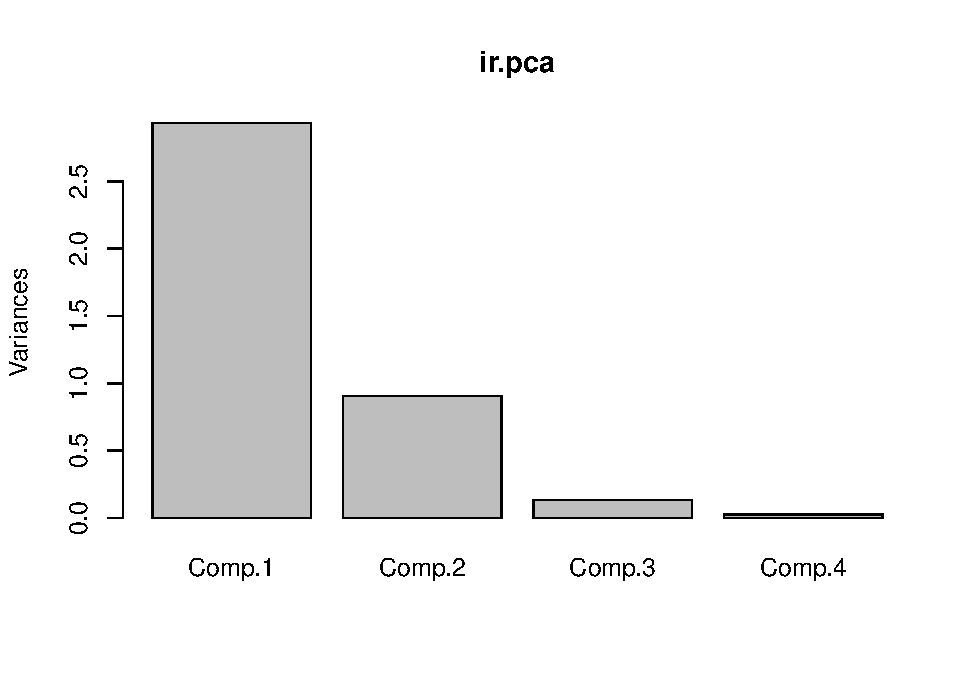
\includegraphics{modern_applied_statistics_CH11_files/figure-latex/unnamed-chunk-3-1.pdf}

\begin{Shaded}
\begin{Highlighting}[]
\CommentTok{\# Crabs data}
\NormalTok{lcrabs }\OtherTok{\textless{}{-}} \FunctionTok{log}\NormalTok{(crabs[, }\DecValTok{4}\SpecialCharTok{:}\DecValTok{8}\NormalTok{])}
\NormalTok{crabs.grp }\OtherTok{\textless{}{-}} \FunctionTok{factor}\NormalTok{(}\FunctionTok{c}\NormalTok{(}\StringTok{"B"}\NormalTok{, }\StringTok{"b"}\NormalTok{, }\StringTok{"O"}\NormalTok{, }\StringTok{"o"}\NormalTok{)[}\FunctionTok{rep}\NormalTok{(}\DecValTok{1}\SpecialCharTok{:}\DecValTok{4}\NormalTok{, }\AttributeTok{each =} \DecValTok{50}\NormalTok{)])}

\CommentTok{\# Principal Component for the crabs data.}
\NormalTok{(lcrabs.pca }\OtherTok{\textless{}{-}} \FunctionTok{princomp}\NormalTok{(lcrabs))}
\end{Highlighting}
\end{Shaded}

\begin{verbatim}
## Call:
## princomp(x = lcrabs)
## 
## Standard deviations:
##    Comp.1    Comp.2    Comp.3    Comp.4    Comp.5 
## 0.5166405 0.0746536 0.0479144 0.0248040 0.0090522 
## 
##  5  variables and  200 observations.
\end{verbatim}

\begin{Shaded}
\begin{Highlighting}[]
\FunctionTok{loadings}\NormalTok{(lcrabs.pca)}
\end{Highlighting}
\end{Shaded}

\begin{verbatim}
## 
## Loadings:
##    Comp.1 Comp.2 Comp.3 Comp.4 Comp.5
## FL  0.452  0.157  0.438  0.752  0.114
## RW  0.387 -0.911                     
## CL  0.453  0.204 -0.371        -0.784
## CW  0.440        -0.672         0.591
## BD  0.497  0.315  0.458 -0.652  0.136
## 
##                Comp.1 Comp.2 Comp.3 Comp.4 Comp.5
## SS loadings       1.0    1.0    1.0    1.0    1.0
## Proportion Var    0.2    0.2    0.2    0.2    0.2
## Cumulative Var    0.2    0.4    0.6    0.8    1.0
\end{verbatim}

\begin{Shaded}
\begin{Highlighting}[]
\NormalTok{lcrabs.pc }\OtherTok{\textless{}{-}} \FunctionTok{predict}\NormalTok{(lcrabs.pca)}
\FunctionTok{dimnames}\NormalTok{(lcrabs.pc) }\OtherTok{\textless{}{-}} \FunctionTok{list}\NormalTok{(}\ConstantTok{NULL}\NormalTok{, }\FunctionTok{paste}\NormalTok{(}\StringTok{"PC"}\NormalTok{, }\DecValTok{1}\SpecialCharTok{:}\DecValTok{5}\NormalTok{, }\AttributeTok{sep =} \StringTok{""}\NormalTok{))}
\end{Highlighting}
\end{Shaded}

\begin{Shaded}
\begin{Highlighting}[]
\CommentTok{\# First two principal components for the crabs data.}
\FunctionTok{eqscplot}\NormalTok{(lcrabs.pc[, }\DecValTok{1}\SpecialCharTok{:}\DecValTok{2}\NormalTok{], }\AttributeTok{type =} \StringTok{"n"}\NormalTok{,}
         \AttributeTok{xlab =} \StringTok{"first principal component"}\NormalTok{,}
         \AttributeTok{ylab =} \StringTok{"second principal component"}\NormalTok{)}
\FunctionTok{text}\NormalTok{(lcrabs.pc[, }\DecValTok{1}\SpecialCharTok{:}\DecValTok{2}\NormalTok{], }\AttributeTok{labels =} \FunctionTok{as.character}\NormalTok{(crabs.grp),}
     \AttributeTok{col =} \DecValTok{3} \SpecialCharTok{+} \FunctionTok{as.integer}\NormalTok{(crabs.grp)) }
\end{Highlighting}
\end{Shaded}

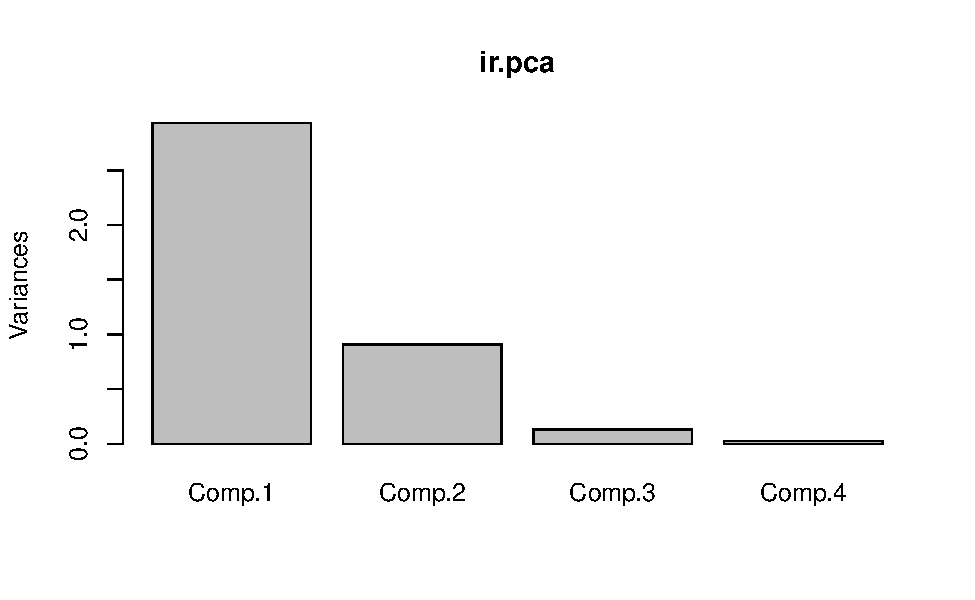
\includegraphics{modern_applied_statistics_CH11_files/figure-latex/unnamed-chunk-5-1.pdf}

\newpage

\hypertarget{distance-methods}{%
\subsubsection{2) Distance methods}\label{distance-methods}}

\begin{Shaded}
\begin{Highlighting}[]
\CommentTok{\# Distance{-}based representations of the iris data}
\NormalTok{ir.scal }\OtherTok{\textless{}{-}} \FunctionTok{cmdscale}\NormalTok{(}\FunctionTok{dist}\NormalTok{(ir) , }\AttributeTok{k =} \DecValTok{2}\NormalTok{, }\AttributeTok{eig =}\NormalTok{ T)}

\NormalTok{distp }\OtherTok{\textless{}{-}} \FunctionTok{dist}\NormalTok{(ir); dist2 }\OtherTok{\textless{}{-}} \FunctionTok{dist}\NormalTok{(ir.scal}\SpecialCharTok{$}\NormalTok{points)}
\FunctionTok{sum}\NormalTok{((distp }\SpecialCharTok{{-}}\NormalTok{ dist2)}\SpecialCharTok{\^{}}\DecValTok{2}\NormalTok{)}\SpecialCharTok{/}\FunctionTok{sum}\NormalTok{(distp}\SpecialCharTok{\^{}}\DecValTok{2}\NormalTok{) }\CommentTok{\# calculating a measure of \textquotesingle{}stress\textquotesingle{}}
\end{Highlighting}
\end{Shaded}

\begin{verbatim}
## [1] 0.0017469
\end{verbatim}

\begin{Shaded}
\begin{Highlighting}[]
\FunctionTok{par}\NormalTok{(}\AttributeTok{mfrow =} \FunctionTok{c}\NormalTok{(}\DecValTok{2}\NormalTok{,}\DecValTok{2}\NormalTok{))}

\FunctionTok{eqscplot}\NormalTok{(ir.scal}\SpecialCharTok{$}\NormalTok{points, }\AttributeTok{type =} \StringTok{"n"}\NormalTok{, }\AttributeTok{main =} \StringTok{"Metric scaling"}\NormalTok{, }\AttributeTok{ratio =} \DecValTok{2}\NormalTok{)}
\FunctionTok{text}\NormalTok{(ir.scal}\SpecialCharTok{$}\NormalTok{points, }\AttributeTok{labels =} \FunctionTok{as.character}\NormalTok{(ir.species), }
     \AttributeTok{col =} \DecValTok{3} \SpecialCharTok{+} \FunctionTok{as.integer}\NormalTok{(ir.species), }\AttributeTok{cex =} \FloatTok{0.8}\NormalTok{)}
\NormalTok{ir.sam }\OtherTok{\textless{}{-}} \FunctionTok{sammon}\NormalTok{(}\FunctionTok{dist}\NormalTok{(ir[}\SpecialCharTok{{-}}\DecValTok{143}\NormalTok{,]))}
\FunctionTok{eqscplot}\NormalTok{(ir.sam}\SpecialCharTok{$}\NormalTok{points, }\AttributeTok{type =} \StringTok{"n"}\NormalTok{, }\AttributeTok{main =} \StringTok{"Sammon mapping"}\NormalTok{, }\AttributeTok{ratio =} \DecValTok{2}\NormalTok{)}
\FunctionTok{text}\NormalTok{(ir.sam}\SpecialCharTok{$}\NormalTok{points, }\AttributeTok{labels =} \FunctionTok{as.character}\NormalTok{(ir.species[}\SpecialCharTok{{-}}\DecValTok{143}\NormalTok{]), }
     \AttributeTok{col =} \DecValTok{3} \SpecialCharTok{+} \FunctionTok{as.integer}\NormalTok{(ir.species), }\AttributeTok{cex =} \FloatTok{0.8}\NormalTok{)}
\NormalTok{ir.iso }\OtherTok{\textless{}{-}} \FunctionTok{isoMDS}\NormalTok{(}\FunctionTok{dist}\NormalTok{(ir[}\SpecialCharTok{{-}}\DecValTok{143}\NormalTok{,]))}
\FunctionTok{eqscplot}\NormalTok{(ir.iso}\SpecialCharTok{$}\NormalTok{points, }\AttributeTok{type =} \StringTok{"n"}\NormalTok{, }\AttributeTok{main =} \StringTok{"Kruskal\textquotesingle{}s MDS"}\NormalTok{, }\AttributeTok{ratio =} \DecValTok{2}\NormalTok{)}
\FunctionTok{text}\NormalTok{(ir.iso}\SpecialCharTok{$}\NormalTok{points, }\AttributeTok{labels =} \FunctionTok{as.character}\NormalTok{(ir.species[}\SpecialCharTok{{-}}\DecValTok{143}\NormalTok{]), }
     \AttributeTok{col =} \DecValTok{3} \SpecialCharTok{+} \FunctionTok{as.integer}\NormalTok{(ir.species), }\AttributeTok{cex =} \FloatTok{0.8}\NormalTok{) }
\end{Highlighting}
\end{Shaded}

\includegraphics{modern_applied_statistics_CH11_files/figure-latex/unnamed-chunk-7-1.pdf}

\newpage

\begin{Shaded}
\begin{Highlighting}[]
\CommentTok{\# Sammon mapping of crabs data}
\NormalTok{cr.scale }\OtherTok{\textless{}{-}} \FloatTok{0.5} \SpecialCharTok{*} \FunctionTok{log}\NormalTok{(crabs}\SpecialCharTok{$}\NormalTok{CL }\SpecialCharTok{*}\NormalTok{ crabs}\SpecialCharTok{$}\NormalTok{CW)}
\NormalTok{slcrabs }\OtherTok{\textless{}{-}}\NormalTok{ lcrabs }\SpecialCharTok{{-}}\NormalTok{ cr.scale}
\NormalTok{cr.means }\OtherTok{\textless{}{-}} \FunctionTok{matrix}\NormalTok{(}\DecValTok{0}\NormalTok{, }\DecValTok{2}\NormalTok{, }\DecValTok{5}\NormalTok{)}
\NormalTok{cr.means[}\DecValTok{1}\NormalTok{,] }\OtherTok{\textless{}{-}} \FunctionTok{colMeans}\NormalTok{(slcrabs[crabs}\SpecialCharTok{$}\NormalTok{sex }\SpecialCharTok{==} \StringTok{"F"}\NormalTok{, ])}
\NormalTok{cr.means[}\DecValTok{2}\NormalTok{,] }\OtherTok{\textless{}{-}} \FunctionTok{colMeans}\NormalTok{(slcrabs [crabs}\SpecialCharTok{$}\NormalTok{sex }\SpecialCharTok{==} \StringTok{"M"}\NormalTok{, ])}
\NormalTok{dslcrabs }\OtherTok{\textless{}{-}}\NormalTok{ slcrabs }\SpecialCharTok{{-}}\NormalTok{ cr.means[}\FunctionTok{as.numeric}\NormalTok{(crabs}\SpecialCharTok{$}\NormalTok{sex),]}
\NormalTok{lcrabs.sam }\OtherTok{\textless{}{-}} \FunctionTok{sammon}\NormalTok{(}\FunctionTok{dist}\NormalTok{(dslcrabs))}
\FunctionTok{eqscplot}\NormalTok{(}\SpecialCharTok{{-}}\NormalTok{lcrabs.sam}\SpecialCharTok{$}\NormalTok{points, }\AttributeTok{type =} \StringTok{"n"}\NormalTok{, }\AttributeTok{xlab =} \StringTok{""}\NormalTok{, }\AttributeTok{ylab =} \StringTok{""}\NormalTok{, }\AttributeTok{tol =} \FloatTok{0.08}\NormalTok{, }\AttributeTok{ratio =} \FloatTok{1.5}\NormalTok{)}
\FunctionTok{text}\NormalTok{(}\SpecialCharTok{{-}}\NormalTok{lcrabs.sam}\SpecialCharTok{$}\NormalTok{points , }\AttributeTok{labels =} \FunctionTok{as.character}\NormalTok{(crabs.grp), }
     \AttributeTok{col =} \FunctionTok{rep}\NormalTok{(}\FunctionTok{c}\NormalTok{(}\StringTok{"blue"}\NormalTok{, }\StringTok{"orange"}\NormalTok{), }\AttributeTok{each =} \DecValTok{100}\NormalTok{))}
\end{Highlighting}
\end{Shaded}

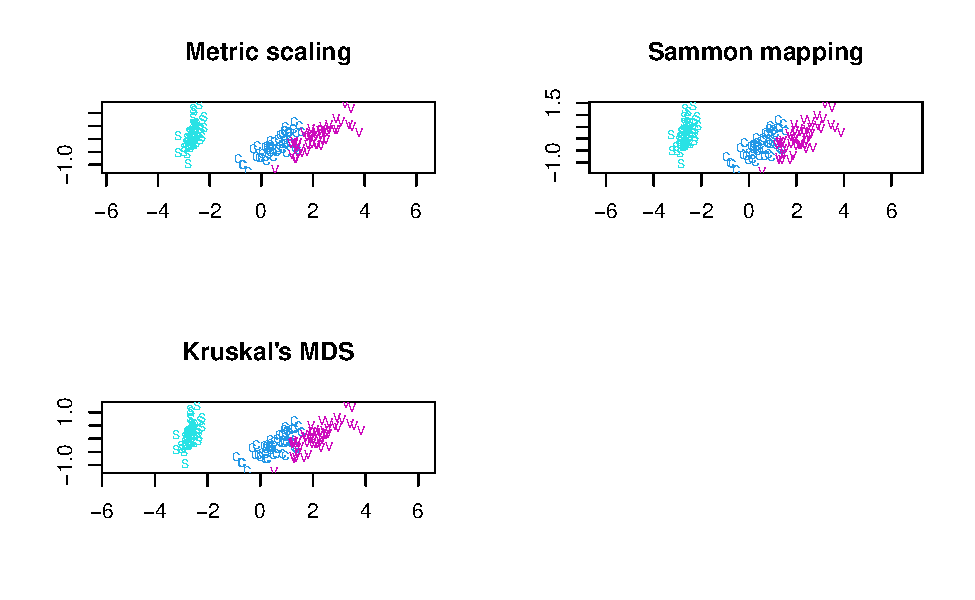
\includegraphics{modern_applied_statistics_CH11_files/figure-latex/unnamed-chunk-8-1.pdf}

\newpage

\begin{Shaded}
\begin{Highlighting}[]
\CommentTok{\# Isotonic multidimensional scaling representation of the fgl data.}
\NormalTok{fgl.iso }\OtherTok{\textless{}{-}} \FunctionTok{isoMDS}\NormalTok{(}\FunctionTok{dist}\NormalTok{(}\FunctionTok{as.matrix}\NormalTok{(fgl[}\SpecialCharTok{{-}}\DecValTok{40}\NormalTok{, }\SpecialCharTok{{-}}\DecValTok{10}\NormalTok{])))}
\FunctionTok{eqscplot}\NormalTok{(fgl.iso}\SpecialCharTok{$}\NormalTok{points, }\AttributeTok{type =} \StringTok{"n"}\NormalTok{, }\AttributeTok{xlab =} \StringTok{""}\NormalTok{, }\AttributeTok{ylab =} \StringTok{""}\NormalTok{, }\AttributeTok{axes =} \ConstantTok{FALSE}\NormalTok{)}
\CommentTok{\# either}
\CommentTok{\# for(i in seq(along = levels(fgl$type))) \{}
\CommentTok{\#   set \textless{}{-} fgl$type[{-}40] == levels(fgl$type)[i]}
\CommentTok{\#   points(fgl.iso$points[set,], pch = 18, cex = 0.6, col = 2 + i)\}}
\CommentTok{\# key(text = list(levels(fgl$type), col = 3:8))}
\CommentTok{\# or}
\FunctionTok{text}\NormalTok{(fgl.iso}\SpecialCharTok{$}\NormalTok{points, }\AttributeTok{labels =} \FunctionTok{c}\NormalTok{(}\StringTok{"F"}\NormalTok{, }\StringTok{"N"}\NormalTok{, }\StringTok{"V"}\NormalTok{, }\StringTok{"C"}\NormalTok{, }\StringTok{"T"}\NormalTok{, }\StringTok{"H"}\NormalTok{)[fgl}\SpecialCharTok{$}\NormalTok{type[}\SpecialCharTok{{-}}\DecValTok{40}\NormalTok{]], }\AttributeTok{cex =} \FloatTok{0.6}\NormalTok{)}
\end{Highlighting}
\end{Shaded}

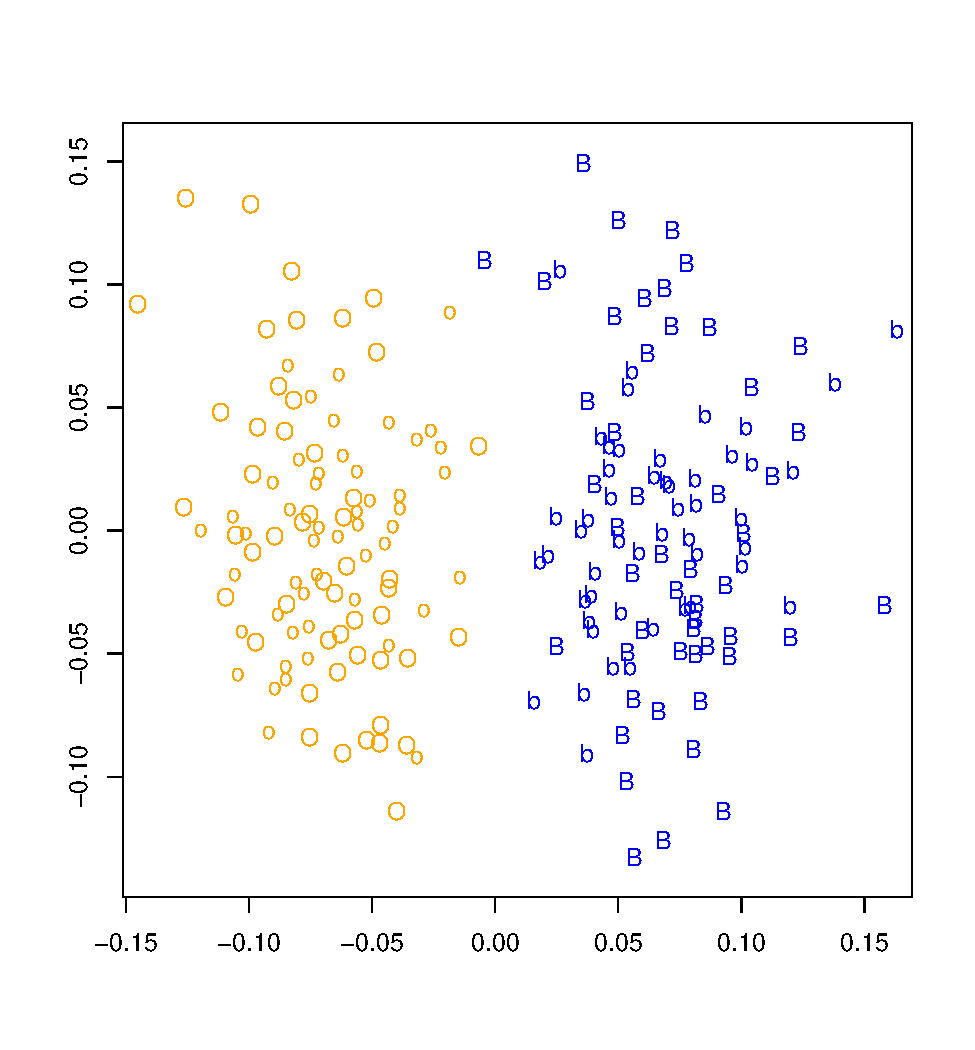
\includegraphics{modern_applied_statistics_CH11_files/figure-latex/unnamed-chunk-9-1.pdf}

\newpage

\hypertarget{self-organizing-maps}{%
\subsubsection{3) Self-organizing maps}\label{self-organizing-maps}}

\begin{Shaded}
\begin{Highlighting}[]
\CommentTok{\# Batch SOM applied to the crabs dataset.}
\FunctionTok{set.seed}\NormalTok{(}\DecValTok{0}\NormalTok{)}
\NormalTok{gr }\OtherTok{\textless{}{-}} \FunctionTok{somgrid}\NormalTok{(}\AttributeTok{topo =} \StringTok{"hexagonal"}\NormalTok{)}
\NormalTok{crabs.som }\OtherTok{\textless{}{-}} \FunctionTok{batchSOM}\NormalTok{(lcrabs, gr, }\FunctionTok{c}\NormalTok{(}\DecValTok{4}\NormalTok{, }\DecValTok{4}\NormalTok{, }\DecValTok{2}\NormalTok{, }\DecValTok{2}\NormalTok{, }\DecValTok{1}\NormalTok{, }\DecValTok{1}\NormalTok{, }\DecValTok{1}\NormalTok{, }\DecValTok{0}\NormalTok{, }\DecValTok{0}\NormalTok{))}

\CommentTok{\# stars plot of the representatives}
\FunctionTok{stars}\NormalTok{(crabs.som}\SpecialCharTok{$}\NormalTok{codes, }\AttributeTok{labels =} \ConstantTok{NULL}\NormalTok{, }\AttributeTok{frame.plot =}\NormalTok{ T)}
\end{Highlighting}
\end{Shaded}


\includegraphics{modern_applied_statistics_CH11_files/figure-latex/unnamed-chunk-10-1.pdf}

\begin{Shaded}
\begin{Highlighting}[]
\FunctionTok{set.seed}\NormalTok{(}\DecValTok{0}\NormalTok{)}

\CommentTok{\# Plot that shows the assignments of the original points}
\NormalTok{bins }\OtherTok{\textless{}{-}} \FunctionTok{as.numeric}\NormalTok{(}\FunctionTok{knn1}\NormalTok{(crabs.som}\SpecialCharTok{$}\NormalTok{code, lcrabs, }\DecValTok{0}\SpecialCharTok{:}\DecValTok{47}\NormalTok{))}
\FunctionTok{plot}\NormalTok{(crabs.som}\SpecialCharTok{$}\NormalTok{grid, }\AttributeTok{type =} \StringTok{"n"}\NormalTok{, }\AttributeTok{frame.plot =}\NormalTok{ T,}
     \AttributeTok{xlim =} \FunctionTok{c}\NormalTok{(}\FunctionTok{min}\NormalTok{(crabs.som}\SpecialCharTok{$}\NormalTok{grid}\SpecialCharTok{$}\NormalTok{pts[,}\DecValTok{1}\NormalTok{])}\SpecialCharTok{{-}}\FloatTok{0.4}\NormalTok{, }\FunctionTok{max}\NormalTok{(crabs.som}\SpecialCharTok{$}\NormalTok{grid}\SpecialCharTok{$}\NormalTok{pts[,}\DecValTok{1}\NormalTok{])}\SpecialCharTok{+}\FloatTok{0.4}\NormalTok{),}
     \AttributeTok{ylim =} \FunctionTok{c}\NormalTok{(}\FunctionTok{min}\NormalTok{(crabs.som}\SpecialCharTok{$}\NormalTok{grid}\SpecialCharTok{$}\NormalTok{pts[,}\DecValTok{2}\NormalTok{])}\SpecialCharTok{{-}}\FloatTok{0.4}\NormalTok{, }\FunctionTok{max}\NormalTok{(crabs.som}\SpecialCharTok{$}\NormalTok{grid}\SpecialCharTok{$}\NormalTok{pts[,}\DecValTok{2}\NormalTok{])}\SpecialCharTok{+}\FloatTok{0.4}\NormalTok{))}
\FunctionTok{symbols}\NormalTok{(crabs.som}\SpecialCharTok{$}\NormalTok{grid}\SpecialCharTok{$}\NormalTok{pts[, }\DecValTok{1}\NormalTok{], crabs.som}\SpecialCharTok{$}\NormalTok{grid}\SpecialCharTok{$}\NormalTok{pts[, }\DecValTok{2}\NormalTok{], }
        \AttributeTok{circles =} \FunctionTok{rep}\NormalTok{(}\FloatTok{0.4}\NormalTok{, }\DecValTok{48}\NormalTok{), }\AttributeTok{inches =} \ConstantTok{FALSE}\NormalTok{, }\AttributeTok{add =} \ConstantTok{TRUE}\NormalTok{)}
\FunctionTok{text}\NormalTok{(crabs.som}\SpecialCharTok{$}\NormalTok{grid}\SpecialCharTok{$}\NormalTok{pts[bins, ] }\SpecialCharTok{+} \FunctionTok{rnorm}\NormalTok{(}\DecValTok{400}\NormalTok{, }\DecValTok{0}\NormalTok{, }\FloatTok{0.1}\NormalTok{), }\FunctionTok{as.character}\NormalTok{(crabs.grp))}
\end{Highlighting}
\end{Shaded}

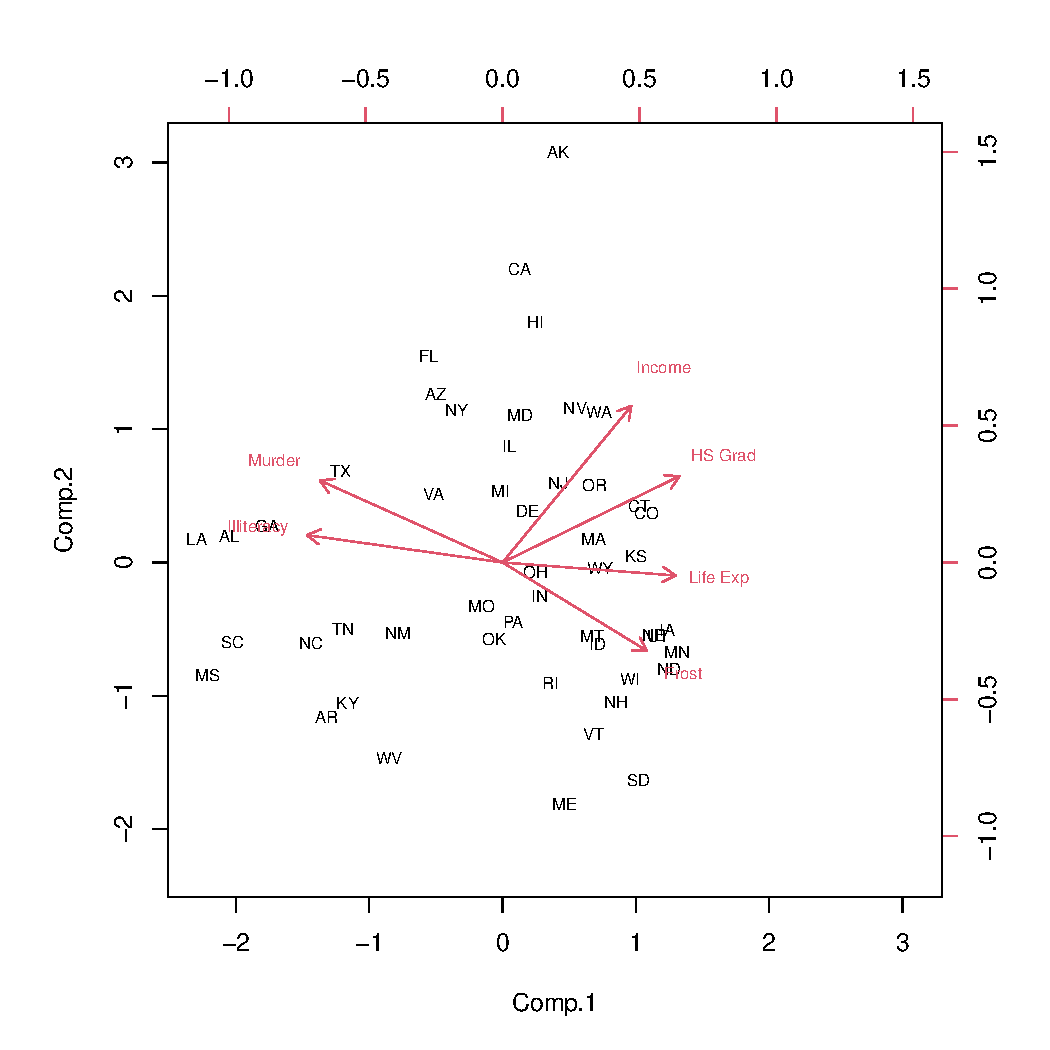
\includegraphics{modern_applied_statistics_CH11_files/figure-latex/unnamed-chunk-11-1.pdf}

\begin{Shaded}
\begin{Highlighting}[]
\FunctionTok{set.seed}\NormalTok{(}\DecValTok{0}\NormalTok{)}

\CommentTok{\# Traditional SOM applied to the crabs dataset.}
\NormalTok{crabs.som2 }\OtherTok{\textless{}{-}} \FunctionTok{SOM}\NormalTok{(lcrabs, gr); }\FunctionTok{stars}\NormalTok{(crabs.som2}\SpecialCharTok{$}\NormalTok{codes, }\AttributeTok{frame.plot =}\NormalTok{ T)}
\end{Highlighting}
\end{Shaded}

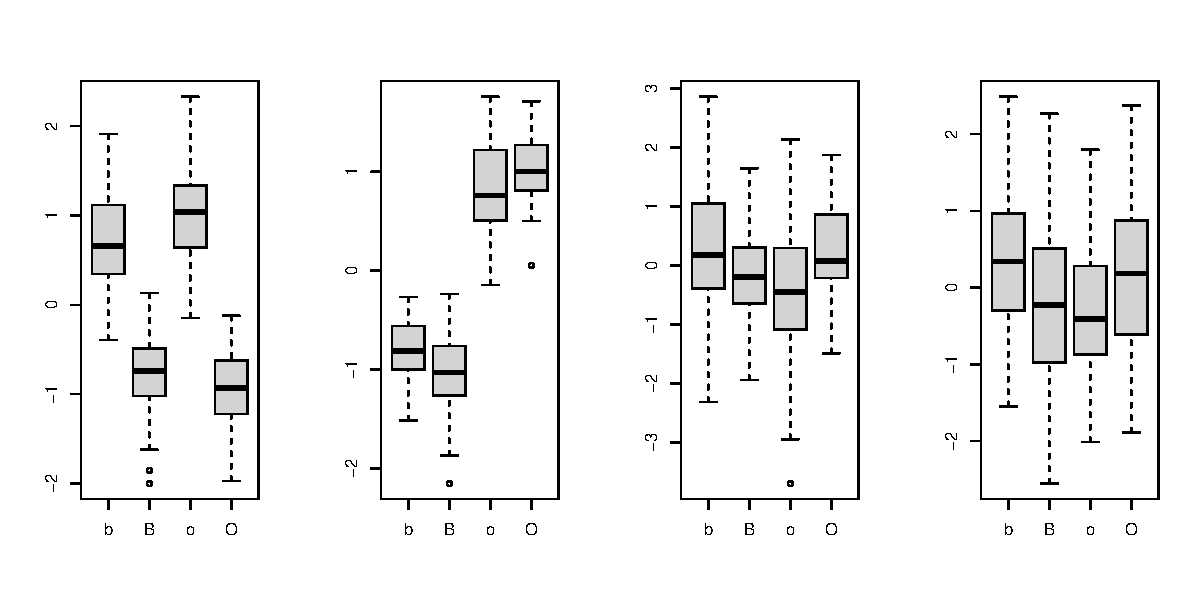
\includegraphics{modern_applied_statistics_CH11_files/figure-latex/unnamed-chunk-12-1.pdf}

\newpage

\hypertarget{biplots}{%
\subsubsection{4) Biplots}\label{biplots}}

\begin{Shaded}
\begin{Highlighting}[]
\CommentTok{\# Principal component biplot of the part of the state.x77 data.}
\NormalTok{state }\OtherTok{\textless{}{-}}\NormalTok{ state.x77[, }\DecValTok{2}\SpecialCharTok{:}\DecValTok{7}\NormalTok{]; }\FunctionTok{row.names}\NormalTok{(state) }\OtherTok{\textless{}{-}}\NormalTok{ state.abb}
\NormalTok{state.pca }\OtherTok{\textless{}{-}} \FunctionTok{princomp}\NormalTok{(state, }\AttributeTok{cor =} \ConstantTok{TRUE}\NormalTok{)}
\NormalTok{state.pca}\SpecialCharTok{$}\NormalTok{loadings[,}\DecValTok{2}\NormalTok{] }\OtherTok{\textless{}{-}} \SpecialCharTok{{-}}\NormalTok{state.pca}\SpecialCharTok{$}\NormalTok{loadings[,}\DecValTok{2}\NormalTok{]}
\NormalTok{state.pca}\SpecialCharTok{$}\NormalTok{scores[,}\DecValTok{2}\NormalTok{] }\OtherTok{\textless{}{-}} \SpecialCharTok{{-}}\NormalTok{state.pca}\SpecialCharTok{$}\NormalTok{scores[,}\DecValTok{2}\NormalTok{]}
\FunctionTok{biplot}\NormalTok{(state.pca, }\AttributeTok{pc.biplot =} \ConstantTok{TRUE}\NormalTok{, }\AttributeTok{cex =} \FloatTok{0.7}\NormalTok{, }\AttributeTok{expand =} \FloatTok{0.8}\NormalTok{)}
\end{Highlighting}
\end{Shaded}

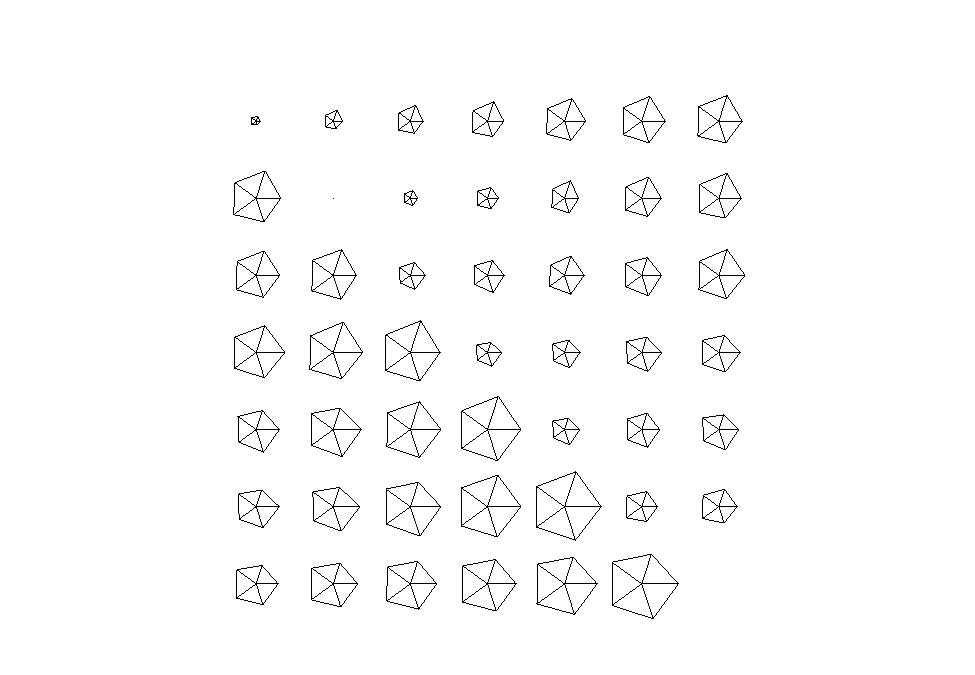
\includegraphics{modern_applied_statistics_CH11_files/figure-latex/unnamed-chunk-13-1.pdf}

\newpage

\hypertarget{independent-component-analysis}{%
\subsubsection{5) Independent component
analysis}\label{independent-component-analysis}}

\begin{Shaded}
\begin{Highlighting}[]
\FunctionTok{set.seed}\NormalTok{(}\DecValTok{0}\NormalTok{)}

\CommentTok{\# Boxplots of four ’signals’ recovered by ICA from the crabs data.}
\NormalTok{nICA }\OtherTok{\textless{}{-}} \DecValTok{4}
\NormalTok{crabs.ica }\OtherTok{\textless{}{-}} \FunctionTok{fastICA}\NormalTok{(crabs[, }\DecValTok{4}\SpecialCharTok{:}\DecValTok{8}\NormalTok{], nICA)}
\NormalTok{Z }\OtherTok{\textless{}{-}}\NormalTok{ crabs.ica}\SpecialCharTok{$}\NormalTok{S}
\FunctionTok{par}\NormalTok{(}\AttributeTok{mfrow =} \FunctionTok{c}\NormalTok{(}\DecValTok{1}\NormalTok{, nICA))}
\ControlFlowTok{for}\NormalTok{(i }\ControlFlowTok{in} \DecValTok{1}\SpecialCharTok{:}\NormalTok{nICA) }\FunctionTok{boxplot}\NormalTok{(Z[, i] }\SpecialCharTok{\textasciitilde{}}\NormalTok{ crabs.grp)}
\end{Highlighting}
\end{Shaded}

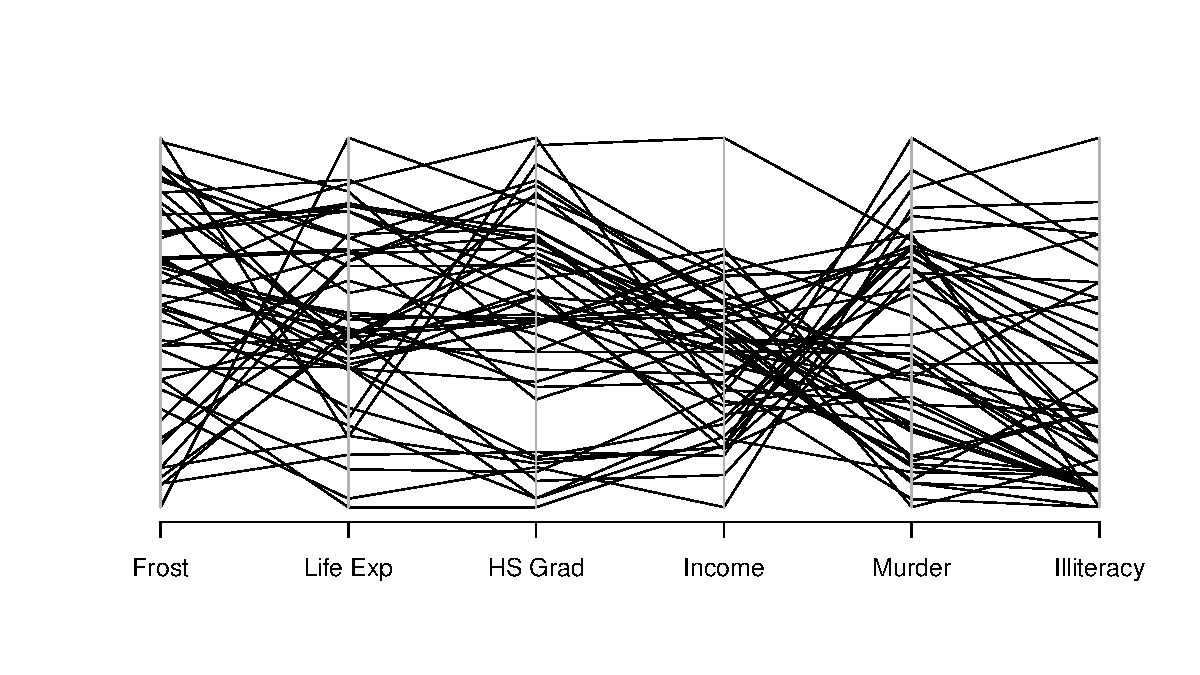
\includegraphics{modern_applied_statistics_CH11_files/figure-latex/unnamed-chunk-14-1.pdf}

\newpage

\hypertarget{glyph-representations}{%
\subsubsection{6) Glyph representations}\label{glyph-representations}}

\begin{Shaded}
\begin{Highlighting}[]
\CommentTok{\# stars plot of the state.x77 dataset.}
\FunctionTok{stars}\NormalTok{(state.x77[, }\FunctionTok{c}\NormalTok{(}\DecValTok{7}\NormalTok{, }\DecValTok{4}\NormalTok{, }\DecValTok{6}\NormalTok{, }\DecValTok{2}\NormalTok{, }\DecValTok{5}\NormalTok{, }\DecValTok{3}\NormalTok{)])}
\end{Highlighting}
\end{Shaded}

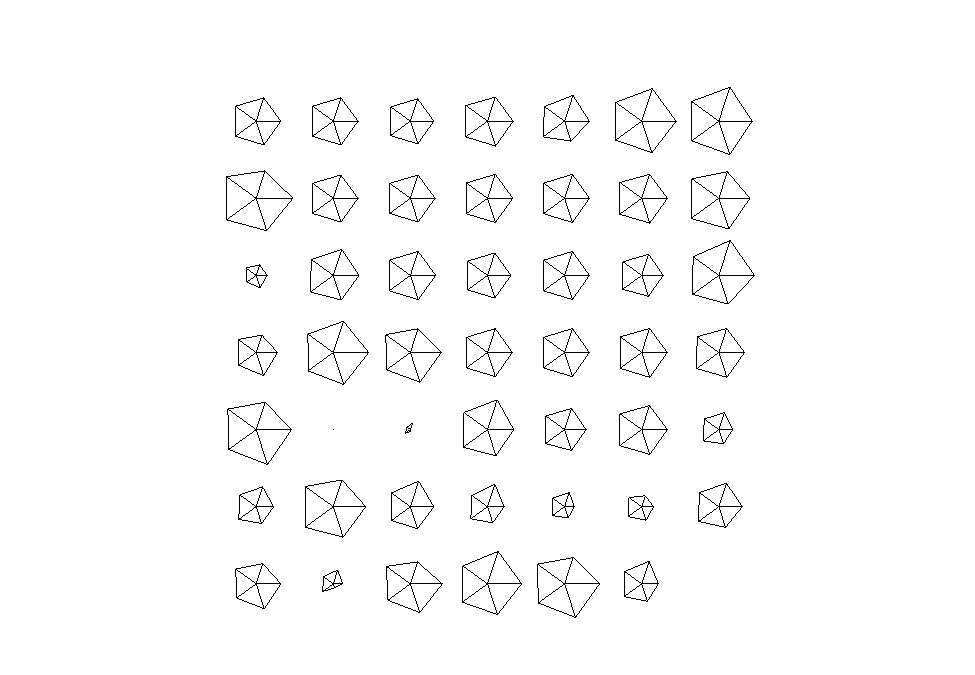
\includegraphics{modern_applied_statistics_CH11_files/figure-latex/unnamed-chunk-15-1.pdf}

\newpage

\hypertarget{parallel-coordinate-plots}{%
\subsubsection{7) Parallel coordinate
plots}\label{parallel-coordinate-plots}}

\begin{Shaded}
\begin{Highlighting}[]
\CommentTok{\# Parallel coordinates plots of the state.x77 dataset.}
\FunctionTok{parcoord}\NormalTok{(state.x77[, }\FunctionTok{c}\NormalTok{(}\DecValTok{7}\NormalTok{, }\DecValTok{4}\NormalTok{, }\DecValTok{6}\NormalTok{, }\DecValTok{2}\NormalTok{, }\DecValTok{5}\NormalTok{, }\DecValTok{3}\NormalTok{)])}
\end{Highlighting}
\end{Shaded}

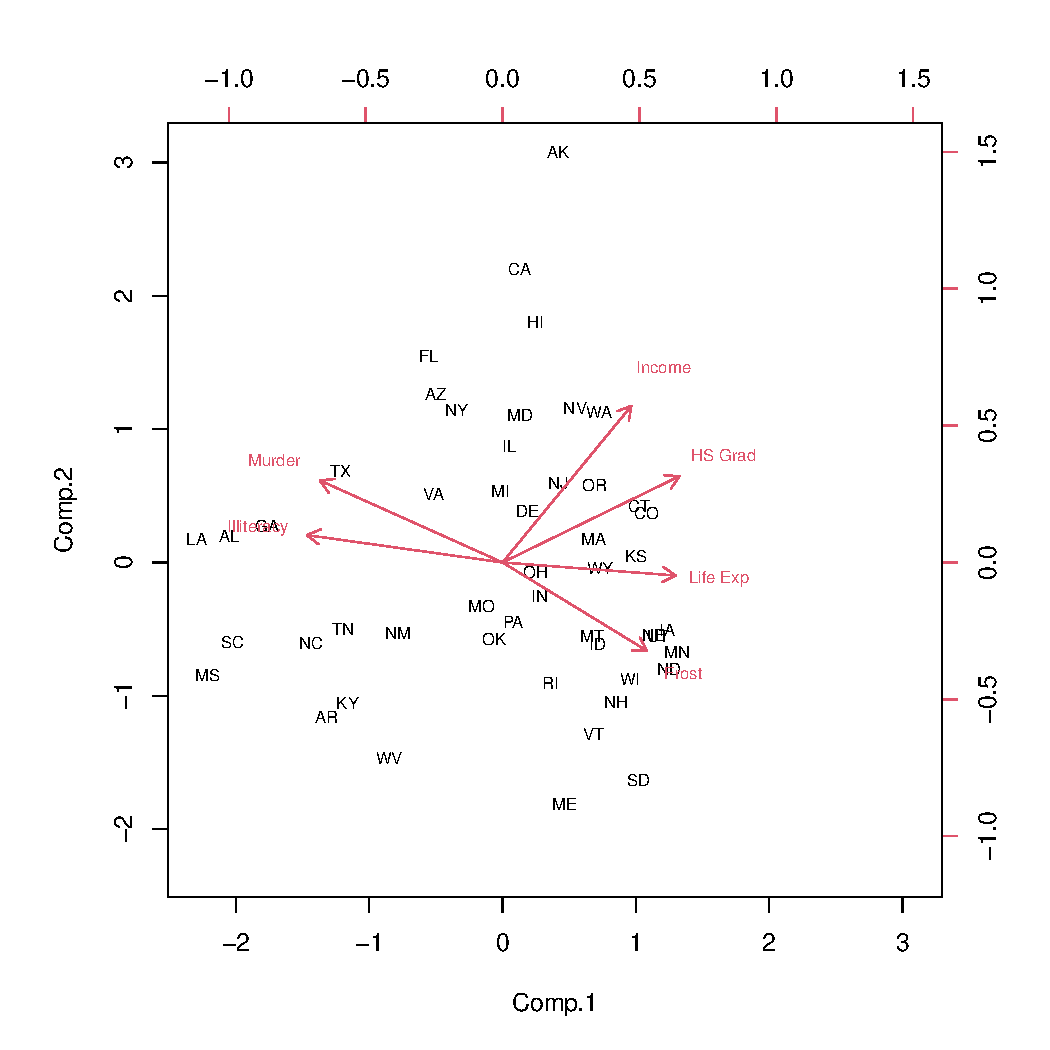
\includegraphics{modern_applied_statistics_CH11_files/figure-latex/unnamed-chunk-16-1.pdf}

\begin{Shaded}
\begin{Highlighting}[]
\CommentTok{\# Parallel coordinates plots of the log{-}transformed iris data}
\FunctionTok{parcoord}\NormalTok{(}\FunctionTok{log}\NormalTok{(ir)[, }\FunctionTok{c}\NormalTok{(}\DecValTok{3}\NormalTok{, }\DecValTok{4}\NormalTok{, }\DecValTok{2}\NormalTok{, }\DecValTok{1}\NormalTok{)], }\AttributeTok{col =} \DecValTok{1} \SpecialCharTok{+}\NormalTok{ (}\DecValTok{0}\SpecialCharTok{:}\DecValTok{149}\NormalTok{)}\SpecialCharTok{\%/\%}\DecValTok{50}\NormalTok{)}
\end{Highlighting}
\end{Shaded}

\includegraphics{modern_applied_statistics_CH11_files/figure-latex/unnamed-chunk-16-2.pdf}

\newpage

\hypertarget{cluster-analysis}{%
\subsection{11.2 Cluster Analysis}\label{cluster-analysis}}

\begin{Shaded}
\begin{Highlighting}[]
\CommentTok{\# Dendograms for the socio{-}economic data on Swiss provinces by single{-}link clustering}
\NormalTok{swiss.x }\OtherTok{\textless{}{-}} \FunctionTok{as.matrix}\NormalTok{(swiss[,}\SpecialCharTok{{-}}\DecValTok{1}\NormalTok{])}
\NormalTok{h }\OtherTok{\textless{}{-}} \FunctionTok{hclust}\NormalTok{(}\FunctionTok{dist}\NormalTok{(swiss.x), }\AttributeTok{method =} \StringTok{"single"}\NormalTok{)}
\FunctionTok{plot}\NormalTok{(h, }\AttributeTok{labels =}\NormalTok{ h}\SpecialCharTok{$}\NormalTok{order, }\AttributeTok{main =} \StringTok{""}\NormalTok{, }\AttributeTok{xlab =} \StringTok{""}\NormalTok{, }\AttributeTok{sub =} \StringTok{""}\NormalTok{)}
\end{Highlighting}
\end{Shaded}

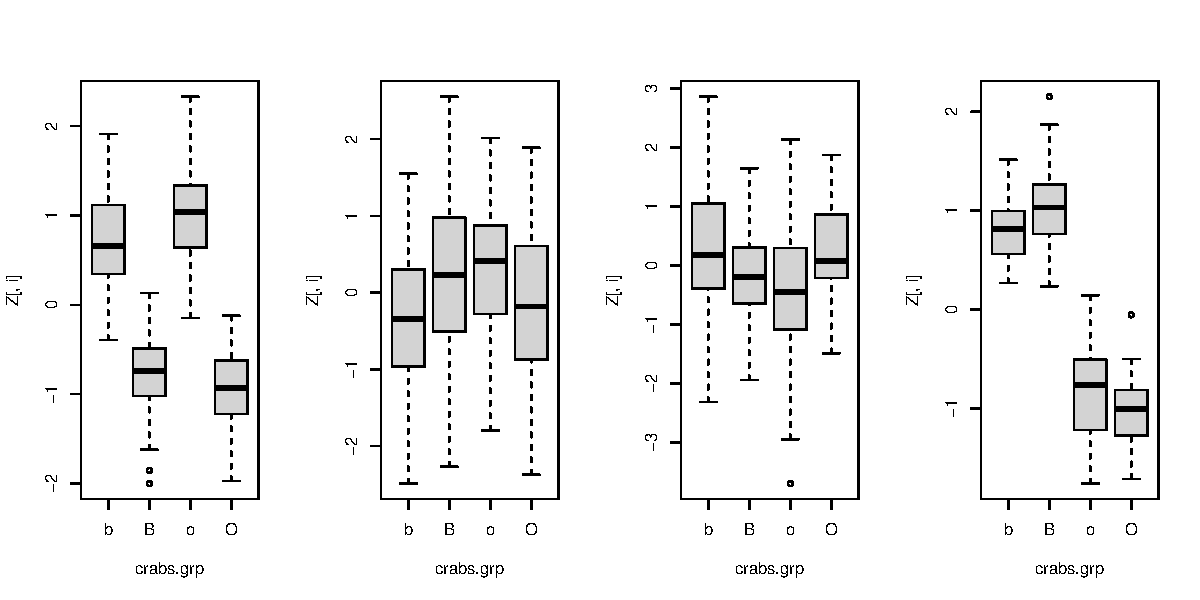
\includegraphics{modern_applied_statistics_CH11_files/figure-latex/unnamed-chunk-17-1.pdf}

\begin{Shaded}
\begin{Highlighting}[]
\CommentTok{\# Dendograms for the socio{-}economic data on Swiss provinces by divisive clustering}
\NormalTok{d }\OtherTok{\textless{}{-}} \FunctionTok{diana}\NormalTok{(swiss.x, )}
\FunctionTok{pltree}\NormalTok{(d, }\AttributeTok{labels =}\NormalTok{ d}\SpecialCharTok{$}\NormalTok{order, }\AttributeTok{main =} \StringTok{""}\NormalTok{, }\AttributeTok{xlab =} \StringTok{""}\NormalTok{, }\AttributeTok{sub =} \StringTok{""}\NormalTok{)}
\end{Highlighting}
\end{Shaded}

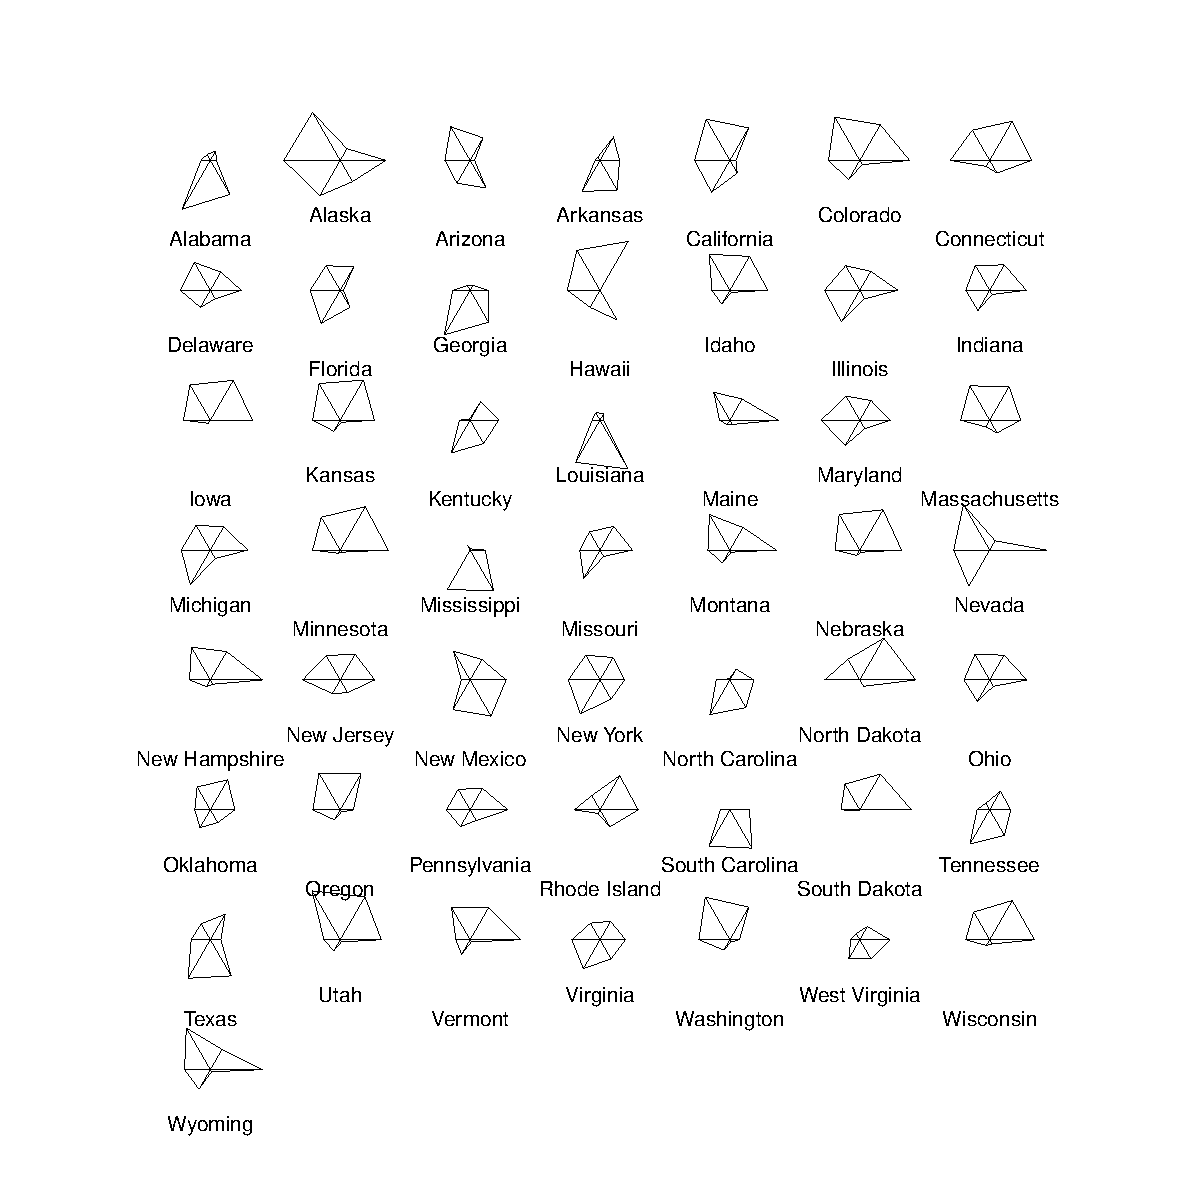
\includegraphics{modern_applied_statistics_CH11_files/figure-latex/unnamed-chunk-18-1.pdf}

\newpage

\begin{Shaded}
\begin{Highlighting}[]
\CommentTok{\# First two principal components for the swiss data }
\CommentTok{\# and labeling by the groups assigned by K{-}means}
\NormalTok{h }\OtherTok{\textless{}{-}} \FunctionTok{hclust}\NormalTok{(}\FunctionTok{dist}\NormalTok{(swiss.x), }\AttributeTok{method =} \StringTok{"average"}\NormalTok{)}
\NormalTok{initial }\OtherTok{\textless{}{-}} \FunctionTok{tapply}\NormalTok{(swiss.x, }\FunctionTok{list}\NormalTok{(}\FunctionTok{rep}\NormalTok{(}\FunctionTok{cutree}\NormalTok{(h, }\DecValTok{3}\NormalTok{), }\FunctionTok{ncol}\NormalTok{(swiss.x)), }\FunctionTok{col}\NormalTok{(swiss.x)), mean)}
\FunctionTok{dimnames}\NormalTok{(initial) }\OtherTok{\textless{}{-}} \FunctionTok{list}\NormalTok{(}\ConstantTok{NULL}\NormalTok{, }\FunctionTok{dimnames}\NormalTok{(swiss.x)[[}\DecValTok{2}\NormalTok{]])}
\NormalTok{km }\OtherTok{\textless{}{-}} \FunctionTok{kmeans}\NormalTok{(swiss.x, initial)}
\NormalTok{(swiss.pca }\OtherTok{\textless{}{-}} \FunctionTok{princomp}\NormalTok{(swiss.x))}
\NormalTok{swiss.px }\OtherTok{\textless{}{-}} \FunctionTok{predict}\NormalTok{(swiss.pca); swiss.px[,}\DecValTok{2}\NormalTok{] }\OtherTok{\textless{}{-}} \SpecialCharTok{{-}}\NormalTok{swiss.px[,}\DecValTok{2}\NormalTok{] }
\FunctionTok{dimnames}\NormalTok{(km}\SpecialCharTok{$}\NormalTok{centers)[[}\DecValTok{2}\NormalTok{]] }\OtherTok{\textless{}{-}} \FunctionTok{dimnames}\NormalTok{(swiss.x)[[}\DecValTok{2}\NormalTok{]]}
\NormalTok{swiss.centers }\OtherTok{\textless{}{-}} \FunctionTok{predict}\NormalTok{(swiss.pca, km}\SpecialCharTok{$}\NormalTok{centers); swiss.centers[,}\DecValTok{2}\NormalTok{] }\OtherTok{\textless{}{-}} \SpecialCharTok{{-}}\NormalTok{swiss.centers[,}\DecValTok{2}\NormalTok{]}
\FunctionTok{eqscplot}\NormalTok{(swiss.px[, }\DecValTok{1}\SpecialCharTok{:}\DecValTok{2}\NormalTok{], }\AttributeTok{type =} \StringTok{"n"}\NormalTok{, }
         \AttributeTok{xlab =} \StringTok{"first principal component"}\NormalTok{ , }\AttributeTok{ylab =} \StringTok{"second principal component"}\NormalTok{)}
\FunctionTok{text}\NormalTok{(swiss.px[, }\DecValTok{1}\SpecialCharTok{:}\DecValTok{2}\NormalTok{], }\AttributeTok{labels =}\NormalTok{ km}\SpecialCharTok{$}\NormalTok{cluster)}
\FunctionTok{points}\NormalTok{(swiss.centers[,}\DecValTok{1}\SpecialCharTok{:}\DecValTok{2}\NormalTok{], }\AttributeTok{pch =} \DecValTok{3}\NormalTok{, }\AttributeTok{cex =} \DecValTok{5}\NormalTok{)}
\FunctionTok{identify}\NormalTok{(swiss.px[, }\DecValTok{1}\SpecialCharTok{:}\DecValTok{2}\NormalTok{], }\AttributeTok{cex =} \FloatTok{0.5}\NormalTok{)}
\end{Highlighting}
\end{Shaded}

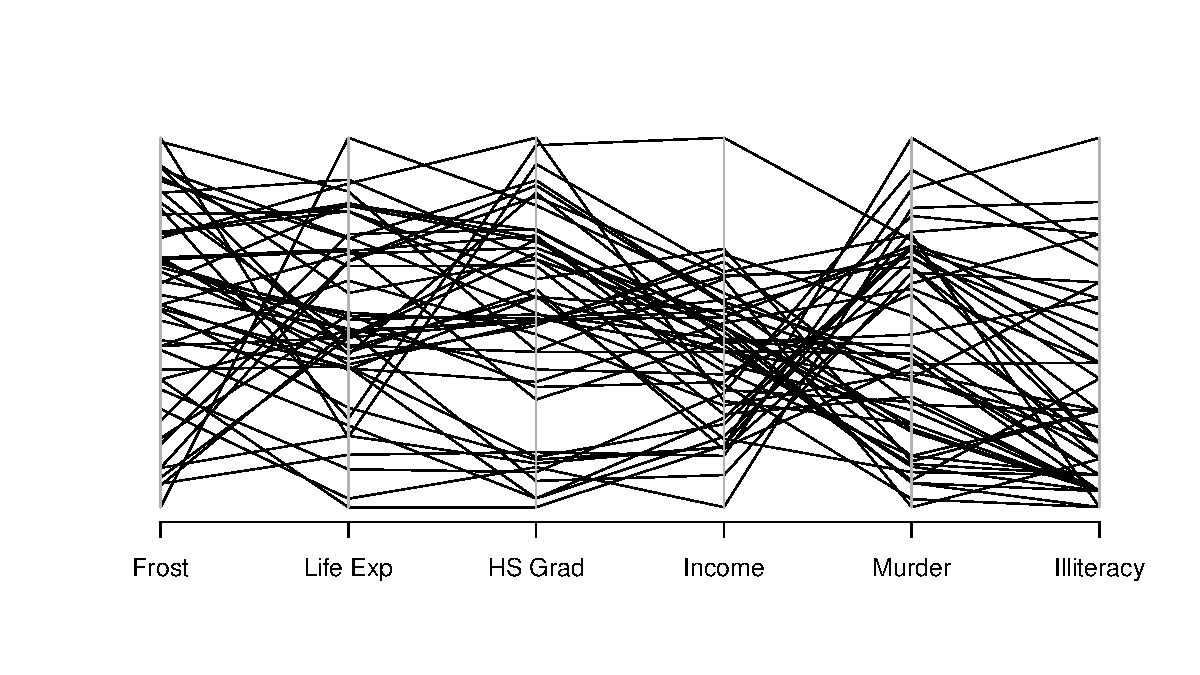
\includegraphics{modern_applied_statistics_CH11_files/figure-latex/unnamed-chunk-19-1.pdf}

\newpage

\begin{Shaded}
\begin{Highlighting}[]
\CommentTok{\# Clusterings of the Swiss provinces data by pam, me, emclust}
\FunctionTok{par}\NormalTok{(}\AttributeTok{mfrow =} \FunctionTok{c}\NormalTok{(}\DecValTok{2}\NormalTok{,}\DecValTok{2}\NormalTok{))}

\NormalTok{swiss.pam }\OtherTok{\textless{}{-}} \FunctionTok{pam}\NormalTok{(swiss.px, }\DecValTok{3}\NormalTok{)}
\FunctionTok{eqscplot}\NormalTok{(swiss.px[, }\DecValTok{1}\SpecialCharTok{:}\DecValTok{2}\NormalTok{], }\AttributeTok{type =} \StringTok{"n"}\NormalTok{,}
         \AttributeTok{xlab =} \StringTok{"first principal component"}\NormalTok{, }\AttributeTok{ylab =} \StringTok{"second principal component"}\NormalTok{,}
         \AttributeTok{main =} \StringTok{"pam"}\NormalTok{)}
\FunctionTok{text}\NormalTok{(swiss.px[,}\DecValTok{1}\SpecialCharTok{:}\DecValTok{2}\NormalTok{], }\AttributeTok{labels =}\NormalTok{ swiss.pam}\SpecialCharTok{$}\NormalTok{clustering)}
\FunctionTok{points}\NormalTok{(swiss.pam}\SpecialCharTok{$}\NormalTok{medoid[,}\DecValTok{1}\SpecialCharTok{:}\DecValTok{2}\NormalTok{], }\AttributeTok{pch =} \DecValTok{3}\NormalTok{, }\AttributeTok{cex =} \DecValTok{3}\NormalTok{)}

\FunctionTok{library}\NormalTok{(mclust)}
\end{Highlighting}
\end{Shaded}

\begin{verbatim}
## Warning: 패키지 'mclust'는 R 버전 4.1.3에서 작성되었습니다
\end{verbatim}

\begin{Shaded}
\begin{Highlighting}[]
\NormalTok{vals }\OtherTok{\textless{}{-}} \FunctionTok{mclustBIC}\NormalTok{(swiss.x)}
\NormalTok{sm }\OtherTok{\textless{}{-}} \FunctionTok{summary}\NormalTok{(vals, swiss.x)}
\FunctionTok{eqscplot}\NormalTok{ (swiss.px [, }\DecValTok{1}\SpecialCharTok{:} \DecValTok{2}\NormalTok{], }\AttributeTok{type =} \StringTok{"n"}\NormalTok{,}
          \AttributeTok{xlab =} \StringTok{"first principal component"}\NormalTok{ , }\AttributeTok{ylab =} \StringTok{"second principal component"}\NormalTok{, }
          \AttributeTok{main =} \StringTok{"emclust"}\NormalTok{)}
\FunctionTok{text}\NormalTok{(swiss.px[, }\DecValTok{1}\SpecialCharTok{:}\DecValTok{2}\NormalTok{], }\AttributeTok{labels =}\NormalTok{ sm}\SpecialCharTok{$}\NormalTok{classification) }

\NormalTok{h }\OtherTok{\textless{}{-}} \FunctionTok{hc}\NormalTok{(}\AttributeTok{modelName =} \StringTok{"VVV"}\NormalTok{, swiss.x)}
\NormalTok{mh }\OtherTok{\textless{}{-}} \FunctionTok{as.vector}\NormalTok{(}\FunctionTok{hclass}\NormalTok{(h, }\DecValTok{3}\NormalTok{))}
\NormalTok{z }\OtherTok{\textless{}{-}} \FunctionTok{me}\NormalTok{(}\AttributeTok{modelName =} \StringTok{"VVV"}\NormalTok{, swiss.x, }\AttributeTok{z =} \FloatTok{0.5}\SpecialCharTok{*}\NormalTok{(}\FunctionTok{unmap}\NormalTok{(mh)}\SpecialCharTok{+}\DecValTok{1}\SpecialCharTok{/}\DecValTok{3}\NormalTok{))}
\FunctionTok{eqscplot}\NormalTok{(swiss.px[, }\DecValTok{1}\SpecialCharTok{:}\DecValTok{2}\NormalTok{], }\AttributeTok{type =} \StringTok{"n"}\NormalTok{, }
         \AttributeTok{xlab =} \StringTok{"first principal component"}\NormalTok{, }\AttributeTok{ylab =} \StringTok{"second principal component"}\NormalTok{,}
         \AttributeTok{main =} \StringTok{"me"}\NormalTok{)}
\FunctionTok{text}\NormalTok{(swiss.px[, }\DecValTok{1}\SpecialCharTok{:}\DecValTok{2}\NormalTok{], }\AttributeTok{labels =} \FunctionTok{max.col}\NormalTok{(z}\SpecialCharTok{$}\NormalTok{z)) }
\end{Highlighting}
\end{Shaded}

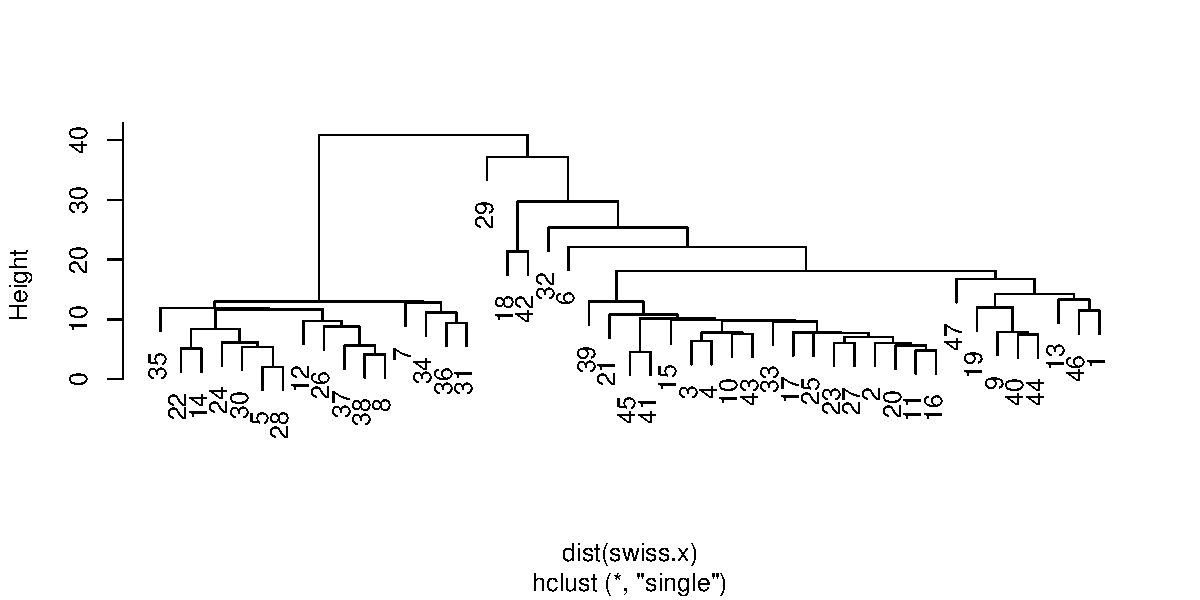
\includegraphics{modern_applied_statistics_CH11_files/figure-latex/unnamed-chunk-20-1.pdf}

\newpage

\hypertarget{factor-analysis}{%
\section{11.3 Factor analysis}\label{factor-analysis}}

\begin{Shaded}
\begin{Highlighting}[]
\NormalTok{ability.FA }\OtherTok{\textless{}{-}} \FunctionTok{factanal}\NormalTok{(}\AttributeTok{covmat =}\NormalTok{ ability.cov, }\AttributeTok{factors =} \DecValTok{1}\NormalTok{)}
\NormalTok{ability.FA}
\end{Highlighting}
\end{Shaded}

\begin{verbatim}
## 
## Call:
## factanal(factors = 1, covmat = ability.cov)
## 
## Uniquenesses:
## general picture  blocks    maze reading   vocab 
##   0.535   0.853   0.748   0.910   0.232   0.280 
## 
## Loadings:
##         Factor1
## general 0.682  
## picture 0.384  
## blocks  0.502  
## maze    0.300  
## reading 0.877  
## vocab   0.849  
## 
##                Factor1
## SS loadings      2.443
## Proportion Var   0.407
## 
## Test of the hypothesis that 1 factor is sufficient.
## The chi square statistic is 75.18 on 9 degrees of freedom.
## The p-value is 1.46e-12
\end{verbatim}

\begin{Shaded}
\begin{Highlighting}[]
\NormalTok{(ability.FA }\OtherTok{\textless{}{-}} \FunctionTok{update}\NormalTok{(ability.FA, }\AttributeTok{factors =} \DecValTok{2}\NormalTok{))}
\end{Highlighting}
\end{Shaded}

\begin{verbatim}
## 
## Call:
## factanal(factors = 2, covmat = ability.cov)
## 
## Uniquenesses:
## general picture  blocks    maze reading   vocab 
##   0.455   0.589   0.218   0.769   0.052   0.334 
## 
## Loadings:
##         Factor1 Factor2
## general 0.499   0.543  
## picture 0.156   0.622  
## blocks  0.206   0.860  
## maze    0.109   0.468  
## reading 0.956   0.182  
## vocab   0.785   0.225  
## 
##                Factor1 Factor2
## SS loadings      1.858   1.724
## Proportion Var   0.310   0.287
## Cumulative Var   0.310   0.597
## 
## Test of the hypothesis that 2 factors are sufficient.
## The chi square statistic is 6.11 on 4 degrees of freedom.
## The p-value is 0.191
\end{verbatim}

\begin{Shaded}
\begin{Highlighting}[]
\CommentTok{\#summary(ability.FA)}
\FunctionTok{round}\NormalTok{(}\FunctionTok{loadings}\NormalTok{(ability.FA) }\SpecialCharTok{\%*\%} \FunctionTok{t}\NormalTok{(}\FunctionTok{loadings}\NormalTok{(ability.FA)) }\SpecialCharTok{+}
        \FunctionTok{diag}\NormalTok{(ability.FA}\SpecialCharTok{$}\NormalTok{uniq), }\DecValTok{3}\NormalTok{)}
\end{Highlighting}
\end{Shaded}

\begin{verbatim}
##         general picture blocks  maze reading vocab
## general   1.000   0.416  0.570 0.308   0.577 0.514
## picture   0.416   1.000  0.567 0.308   0.262 0.262
## blocks    0.570   0.567  1.000 0.425   0.353 0.355
## maze      0.308   0.308  0.425 1.000   0.189 0.190
## reading   0.577   0.262  0.353 0.189   1.000 0.791
## vocab     0.514   0.262  0.355 0.190   0.791 1.000
\end{verbatim}

\begin{Shaded}
\begin{Highlighting}[]
\CommentTok{\# Factor rotations}
\FunctionTok{library}\NormalTok{(GPArotation)}
\end{Highlighting}
\end{Shaded}

\begin{verbatim}
## Warning: 패키지 'GPArotation'는 R 버전 4.1.3에서 작성되었습니다
\end{verbatim}

\begin{Shaded}
\begin{Highlighting}[]
\NormalTok{L }\OtherTok{\textless{}{-}} \FunctionTok{loadings}\NormalTok{(ability.FA)}
\FunctionTok{print}\NormalTok{(oblirot }\OtherTok{\textless{}{-}} \FunctionTok{oblimin}\NormalTok{(L))}
\end{Highlighting}
\end{Shaded}

\begin{verbatim}
## Oblique rotation method Oblimin Quartimin converged.
## Loadings:
##         Factor1 Factor2
## general  0.3864  0.4745
## picture -0.0110  0.6459
## blocks  -0.0263  0.8961
## maze    -0.0180  0.4883
## reading  0.9901 -0.0371
## vocab    0.7906  0.0526
## 
## Rotating matrix:
##        [,1]   [,2]
## [1,]  1.091 -0.249
## [2,] -0.292  1.102
## 
## Phi:
##       [,1]  [,2]
## [1,] 1.000 0.465
## [2,] 0.465 1.000
\end{verbatim}

\begin{Shaded}
\begin{Highlighting}[]
\FunctionTok{par}\NormalTok{(}\AttributeTok{pty =} \StringTok{"s"}\NormalTok{)}
\FunctionTok{eqscplot}\NormalTok{(L, }\AttributeTok{xlim =} \FunctionTok{c}\NormalTok{(}\DecValTok{0}\NormalTok{,}\DecValTok{1}\NormalTok{), }\AttributeTok{ylim =} \FunctionTok{c}\NormalTok{(}\DecValTok{0}\NormalTok{,}\DecValTok{1}\NormalTok{))}
\ControlFlowTok{if}\NormalTok{(}\FunctionTok{interactive}\NormalTok{()) }\FunctionTok{identify}\NormalTok{(L[}\DecValTok{1}\SpecialCharTok{:}\DecValTok{6}\NormalTok{,}\DecValTok{1}\NormalTok{], }\FunctionTok{dimnames}\NormalTok{(L)[[}\DecValTok{1}\NormalTok{]])}
\NormalTok{naxes }\OtherTok{\textless{}{-}}\NormalTok{ oblirot}\SpecialCharTok{$}\NormalTok{Th}
\FunctionTok{arrows}\NormalTok{(}\FunctionTok{rep}\NormalTok{(}\DecValTok{0}\NormalTok{, }\DecValTok{2}\NormalTok{), }\FunctionTok{rep}\NormalTok{(}\DecValTok{0}\NormalTok{, }\DecValTok{2}\NormalTok{), naxes[,}\DecValTok{1}\NormalTok{], naxes[,}\DecValTok{2}\NormalTok{])}
\FunctionTok{text}\NormalTok{(L[}\DecValTok{1}\SpecialCharTok{:}\DecValTok{6}\NormalTok{,}\DecValTok{1}\SpecialCharTok{:}\DecValTok{2}\NormalTok{], }\FunctionTok{dimnames}\NormalTok{(L)[[}\DecValTok{1}\NormalTok{]])}
\end{Highlighting}
\end{Shaded}

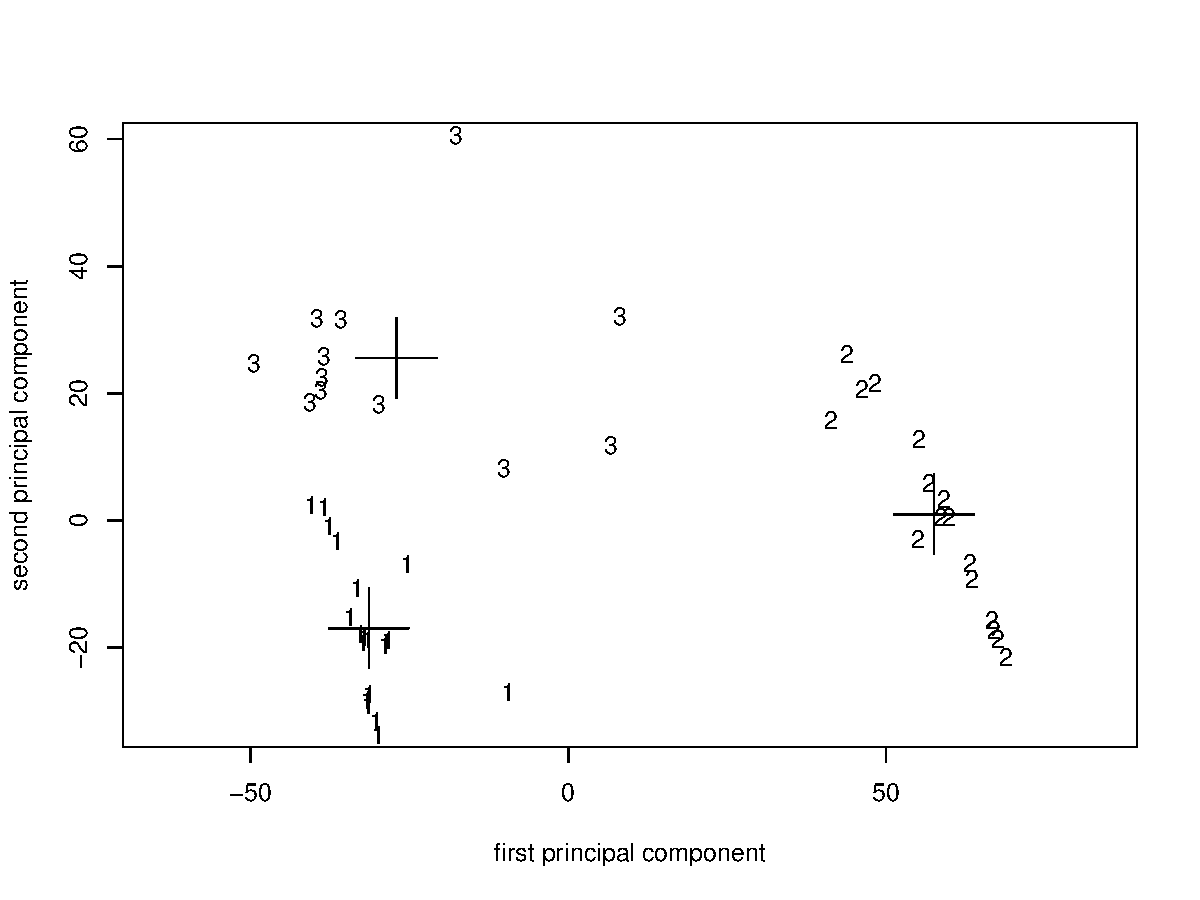
\includegraphics{modern_applied_statistics_CH11_files/figure-latex/unnamed-chunk-22-1.pdf}

\hypertarget{discrete-multivariate-analysis}{%
\section{11.4 Discrete multivariate
analysis}\label{discrete-multivariate-analysis}}

\hypertarget{mosaic-plot}{%
\subsection{mosaic plot}\label{mosaic-plot}}

\begin{Shaded}
\begin{Highlighting}[]
\FunctionTok{par}\NormalTok{(}\AttributeTok{mfrow =} \FunctionTok{c}\NormalTok{(}\DecValTok{2}\NormalTok{,}\DecValTok{1}\NormalTok{))}
\CommentTok{\# Mosaic plots for Fisher\textquotesingle{}s data on people from Caithness}
\NormalTok{caith }\OtherTok{\textless{}{-}} \FunctionTok{as.matrix}\NormalTok{(caith)}
\FunctionTok{names}\NormalTok{(}\FunctionTok{dimnames}\NormalTok{(caith)) }\OtherTok{\textless{}{-}} \FunctionTok{c}\NormalTok{(}\StringTok{"eyes"}\NormalTok{, }\StringTok{"hair"}\NormalTok{)}
\FunctionTok{mosaicplot}\NormalTok{(caith, }\AttributeTok{color =} \ConstantTok{TRUE}\NormalTok{)}
\CommentTok{\# Mosaic plots for Copenhagen housing satisfaction data}
\NormalTok{House }\OtherTok{\textless{}{-}} \FunctionTok{xtabs}\NormalTok{(Freq }\SpecialCharTok{\textasciitilde{}}\NormalTok{ Type }\SpecialCharTok{+}\NormalTok{ Infl }\SpecialCharTok{+}\NormalTok{ Cont }\SpecialCharTok{+}\NormalTok{ Sat, housing)}
\FunctionTok{mosaicplot}\NormalTok{(House, }\AttributeTok{color =} \ConstantTok{TRUE}\NormalTok{)}
\end{Highlighting}
\end{Shaded}

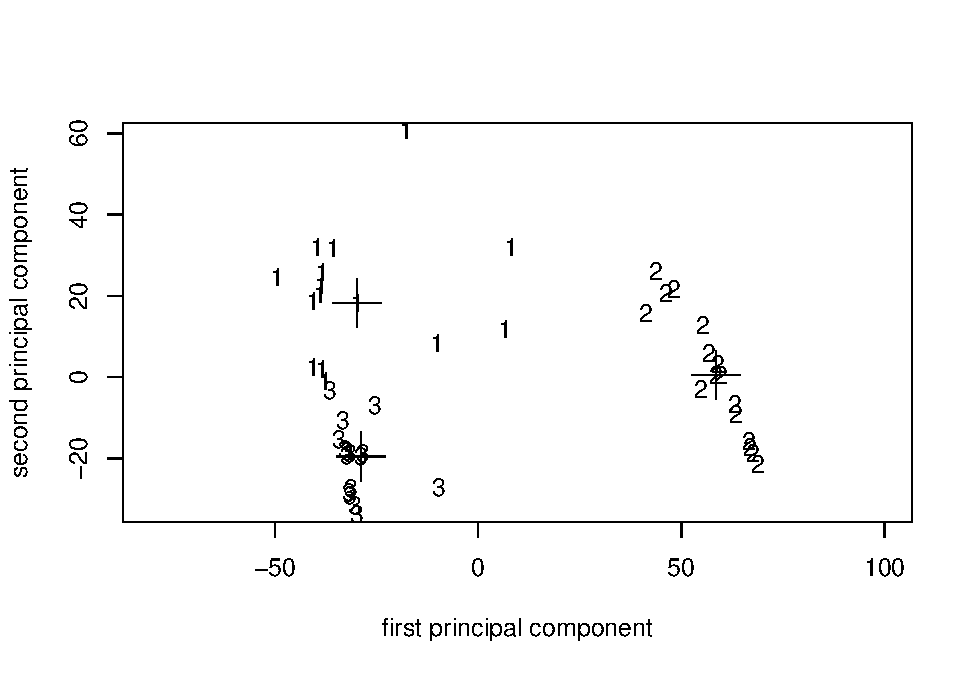
\includegraphics{modern_applied_statistics_CH11_files/figure-latex/unnamed-chunk-23-1.pdf}

\newpage

\begin{Shaded}
\begin{Highlighting}[]
\CommentTok{\# Three variants of correspondence analysis plots from Fisher\textquotesingle{}s data}
\NormalTok{caith2 }\OtherTok{\textless{}{-}}\NormalTok{ caith}
\FunctionTok{dimnames}\NormalTok{(caith2)[[}\DecValTok{2}\NormalTok{]] }\OtherTok{\textless{}{-}} \FunctionTok{c}\NormalTok{(}\StringTok{"F"}\NormalTok{, }\StringTok{"R"}\NormalTok{, }\StringTok{"M"}\NormalTok{, }\StringTok{"D"}\NormalTok{, }\StringTok{"B"}\NormalTok{)}
\FunctionTok{par}\NormalTok{(}\AttributeTok{mfcol =} \FunctionTok{c}\NormalTok{(}\DecValTok{1}\NormalTok{, }\DecValTok{3}\NormalTok{))}
\FunctionTok{plot}\NormalTok{(}\FunctionTok{corresp}\NormalTok{(caith2, }\AttributeTok{nf =} \DecValTok{2}\NormalTok{)); }\FunctionTok{title}\NormalTok{(}\StringTok{"symmetric"}\NormalTok{)}
\FunctionTok{plot}\NormalTok{(}\FunctionTok{corresp}\NormalTok{(caith2, }\AttributeTok{nf =} \DecValTok{2}\NormalTok{), }\AttributeTok{type =} \StringTok{"rows"}\NormalTok{); }\FunctionTok{title}\NormalTok{(}\StringTok{"rows"}\NormalTok{)}
\FunctionTok{plot}\NormalTok{(}\FunctionTok{corresp}\NormalTok{(caith2, }\AttributeTok{nf =} \DecValTok{2}\NormalTok{), }\AttributeTok{type =} \StringTok{"col"}\NormalTok{); }\FunctionTok{title}\NormalTok{(}\StringTok{"columns"}\NormalTok{)}
\end{Highlighting}
\end{Shaded}

\includegraphics{modern_applied_statistics_CH11_files/figure-latex/unnamed-chunk-24-1.pdf}

\begin{Shaded}
\begin{Highlighting}[]
\CommentTok{\# Multiple correspondence analysis plot of dataset farms}
\NormalTok{farms.mca }\OtherTok{\textless{}{-}} \FunctionTok{mca}\NormalTok{(farms, }\AttributeTok{abbrev =} \ConstantTok{TRUE}\NormalTok{)  }\CommentTok{\# Use levels as names}
\FunctionTok{plot}\NormalTok{(farms.mca, }\AttributeTok{cex =} \FunctionTok{rep}\NormalTok{(}\FloatTok{0.7}\NormalTok{, }\DecValTok{2}\NormalTok{))}
\end{Highlighting}
\end{Shaded}

\includegraphics{modern_applied_statistics_CH11_files/figure-latex/unnamed-chunk-25-1.pdf}

\end{document}
